% MEI impedance meter, SIMPLIFIED version: current-sense divider (no bridge modules).
% Compile: pdflatex mei_circuit_divider.tex
\documentclass[border=12pt]{standalone}
\usepackage[american]{circuitikz}
\usepackage{amsmath}
\usetikzlibrary{calc}
\ctikzset{bipoles/length=1.5cm}
\tikzset{every picture/.append style={font=\small}}

% voltage follower: name, x of (+) input, y of (+) input, label, feedback drop (cm)
\newcommand{\follower}[5]{%
  \node[op amp, noinv input up, anchor=+] (#1) at (#2,#3) {};
  \node[font=\scriptsize, align=center] at ([yshift=0.7cm]#1.up) {#4};
  \coordinate (#1o) at ($(#1.out)+(0.8,0)$);
  \coordinate (#1l) at ($(#1.-)+(-0.6,-#5)$);
  \draw (#1.out) -- (#1o) -- (#1o |- #1l) -- (#1l) -- (#1l |- #1.-) -- (#1.-);
  \fill (#1o) circle (1.4pt);
}

\begin{document}
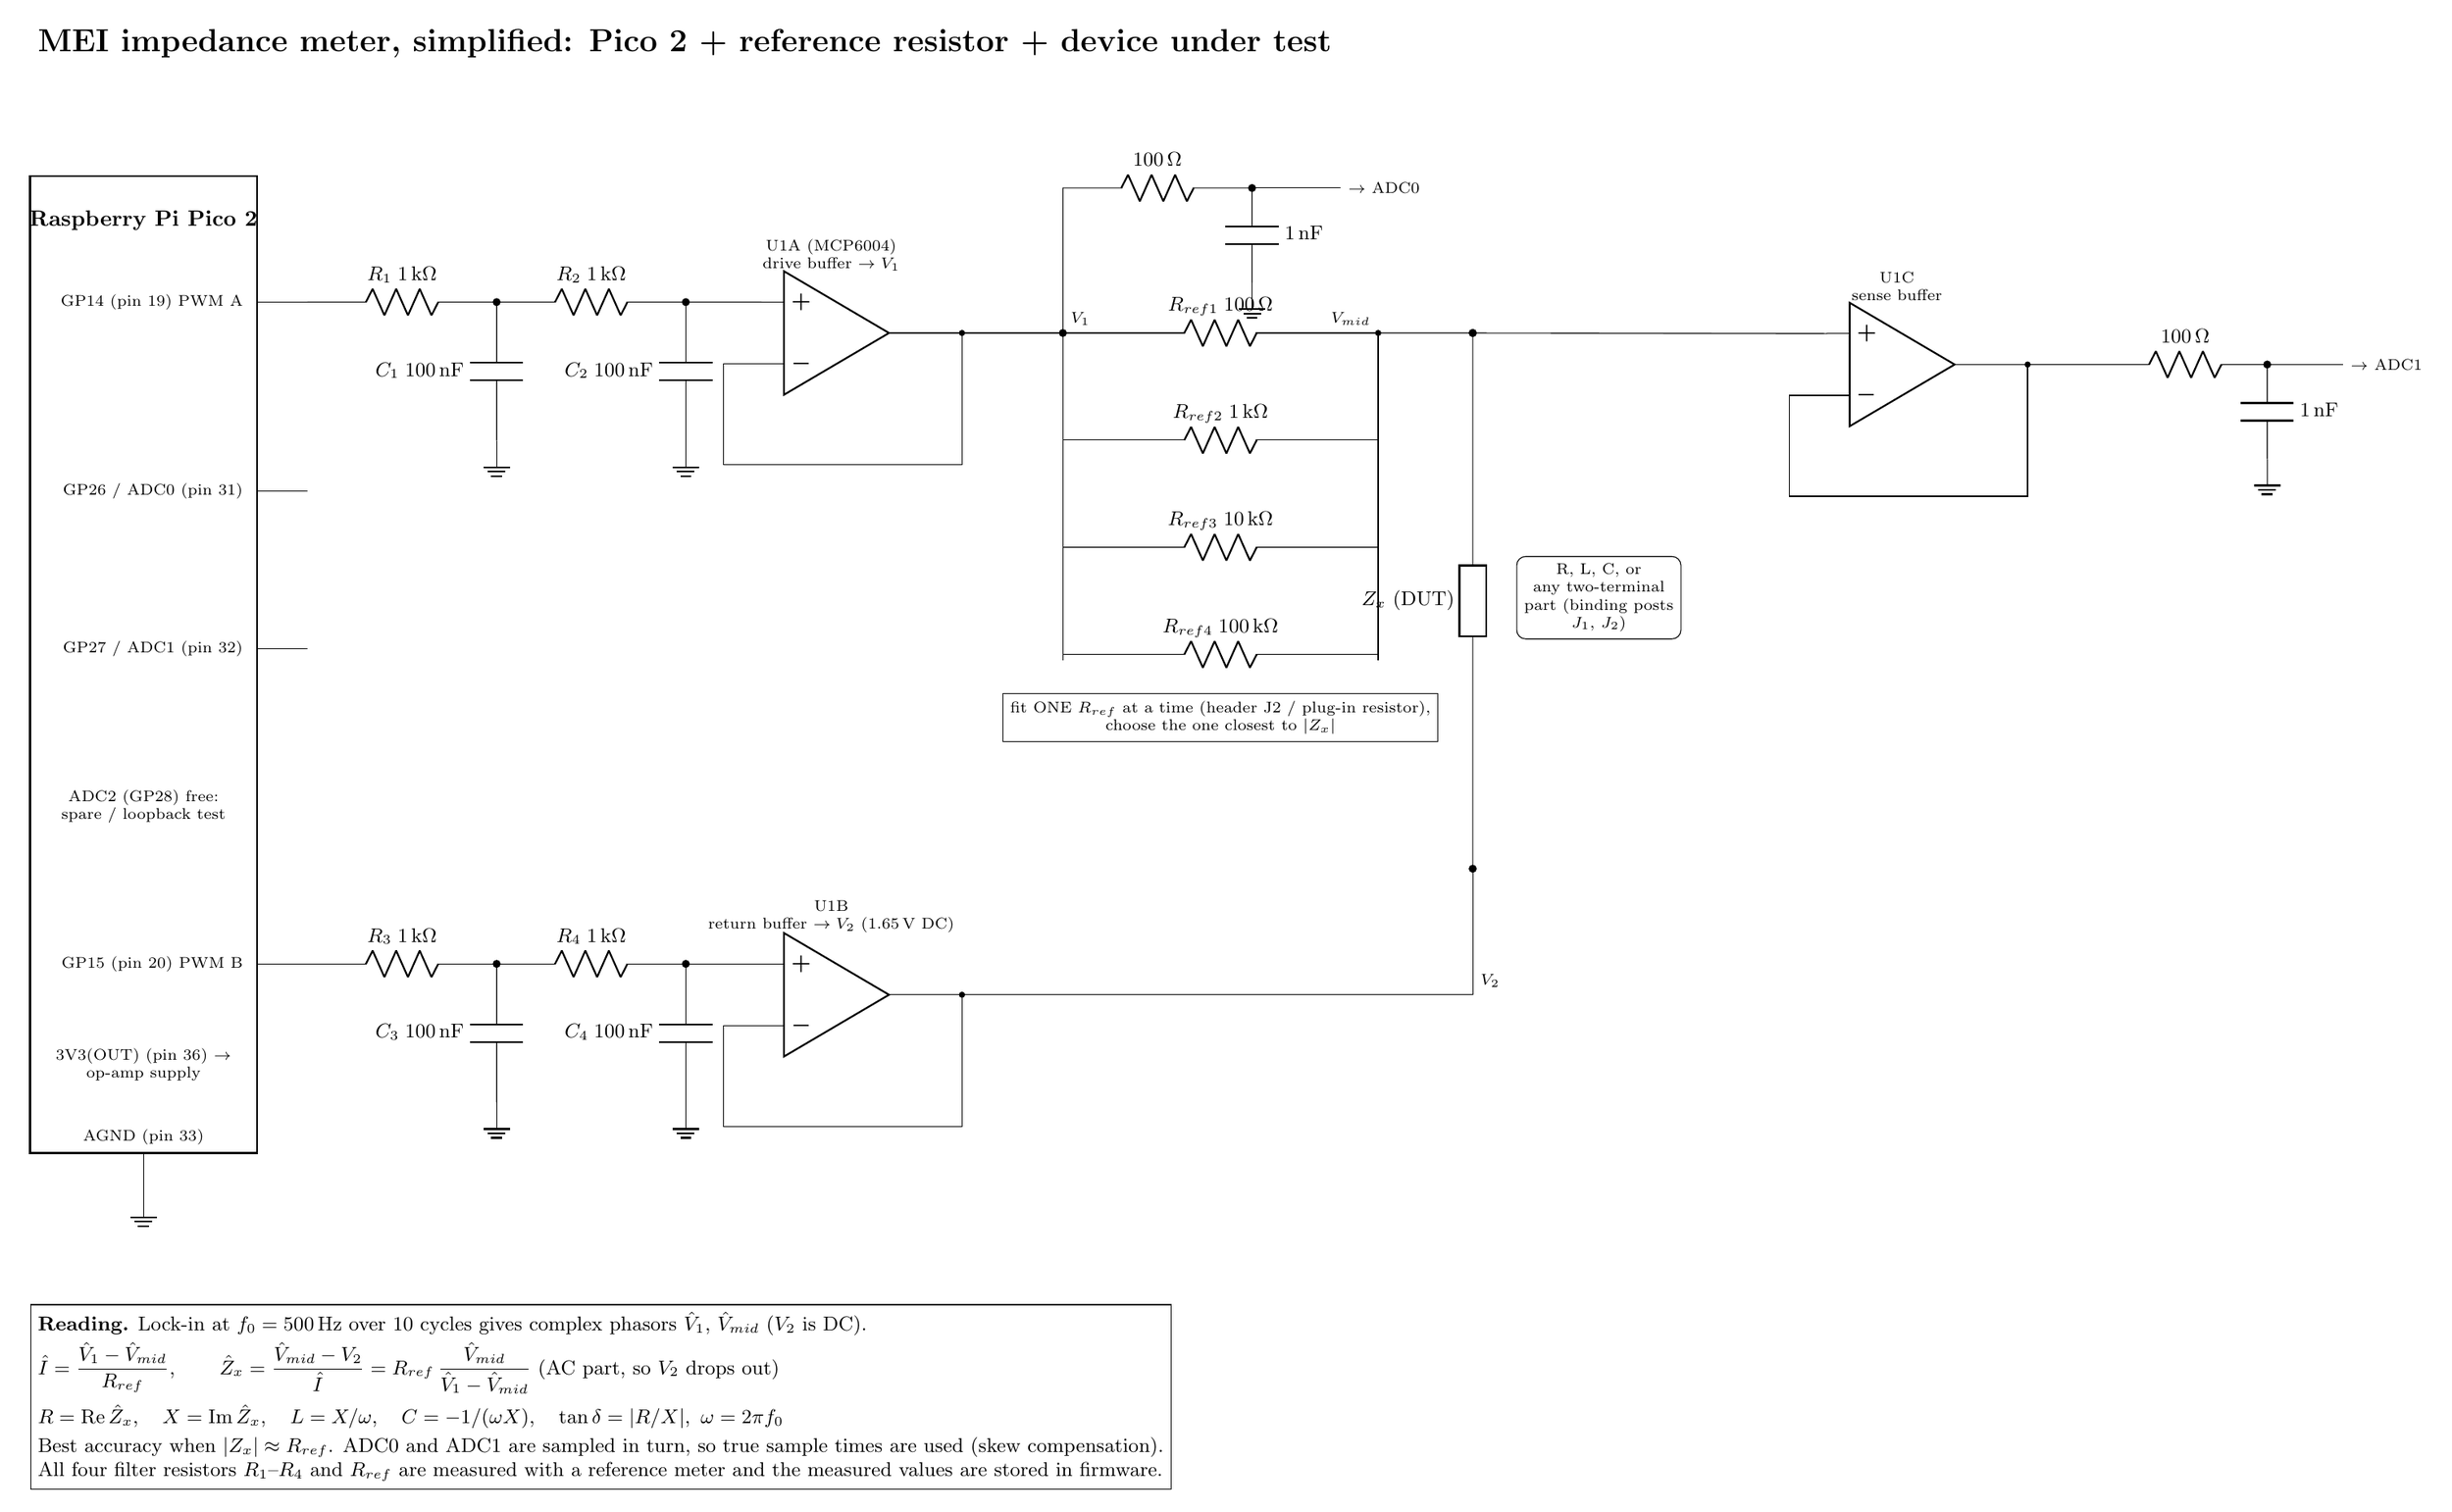
\begin{tikzpicture}
\node[font=\Large\bfseries, anchor=west] at (0,8.6)
  {MEI impedance meter, simplified: Pico 2 + reference resistor + device under test};

% ---------------- Pico 2 ----------------
\draw[thick] (0,-9) rectangle (3.6,6.5);
\node[font=\bfseries] at (1.8,5.8) {Raspberry Pi Pico 2};
\foreach \y/\txt in {4.5/{GP14 (pin 19)  PWM A}, -6/{GP15 (pin 20)  PWM B},
                     6.2/{}, 1.5/{GP26 / ADC0 (pin 31)}, -1/{GP27 / ADC1 (pin 32)}}{
  \ifx\txt\empty\else
  \node[left,font=\scriptsize] at (3.5,\y) {\txt};
  \draw (3.6,\y) -- (4.4,\y);\fi}
\node[font=\scriptsize,align=center] at (1.8,-3.5) {ADC2 (GP28) free:\\ spare / loopback test};
\draw (1.8,-9) -- (1.8,-9.6) node[ground]{};
\node[above,font=\scriptsize] at (1.8,-9) {AGND (pin 33)};
\node[font=\scriptsize,align=center] at (1.8,-7.6) {3V3(OUT) (pin 36) $\to$\\ op-amp supply};

% ---------------- Channel A: PWM A -> RC -> RC -> follower U1A -> V1 ----------------
\draw (4.4,4.5) to[R, l=$R_1\;1\,\mathrm{k\Omega}$] (7.4,4.5) node[circ]{} coordinate(a1)
      to[R, l=$R_2\;1\,\mathrm{k\Omega}$] (10.4,4.5) node[circ]{} coordinate(a2) -- (11.6,4.5);
\draw (a1) to[C, l_=$C_1\;100\,\mathrm{nF}$] ++(0,-2.2) node[ground]{};
\draw (a2) to[C, l_=$C_2\;100\,\mathrm{nF}$] ++(0,-2.2) node[ground]{};
\follower{A1}{11.6}{4.5}{U1A (MCP6004)\\ drive buffer $\to V_1$}{1.6}

% ---------------- Channel B: PWM B (50 % duty) -> RC -> RC -> follower U1B -> V2 (mid-rail) ----
\draw (4.4,-6) to[R, l=$R_3\;1\,\mathrm{k\Omega}$] (7.4,-6) node[circ]{} coordinate(b1)
      to[R, l=$R_4\;1\,\mathrm{k\Omega}$] (10.4,-6) node[circ]{} coordinate(b2) -- (11.6,-6);
\draw (b1) to[C, l_=$C_3\;100\,\mathrm{nF}$] ++(0,-2.2) node[ground]{};
\draw (b2) to[C, l_=$C_4\;100\,\mathrm{nF}$] ++(0,-2.2) node[ground]{};
\follower{A2}{11.6}{-6}{U1B\\ return buffer $\to V_2$ (1.65\,V DC)}{1.6}

% ---------------- V1 node and ADC0 tap ----------------
\draw (A1o) -- ++(1.6,0) coordinate(V1) node[circ]{};
\node[above right,font=\scriptsize] at (V1) {$V_1$};
\draw (V1) -- ++(0,2.3) to[R, l=$100\,\Omega$] ++(3,0) node[circ]{} coordinate(n0)
      to[C, l=$1\,\mathrm{nF}$] ++(0,-1.5) node[ground]{};
\draw (n0) -- ++(1.4,0) node[right,font=\scriptsize]{$\to$ ADC0};

% ---------------- Reference resistor ranges (fit ONE) ----------------
\coordinate (Vm) at ($(V1)+(5,0)$);
\draw (V1) -- ++(0,-5.2);
\draw (Vm) -- ++(0,-5.2);
\draw (V1) to[R, l=$R_{ref1}\;100\,\Omega$] (Vm);
\foreach \k/\val in {1/{1\,\mathrm{k\Omega}},2/{10\,\mathrm{k\Omega}},3/{100\,\mathrm{k\Omega}}}{
  \draw ($(V1)+(0,-1.7*\k)$) to[R, l=$R_{ref\the\numexpr\k+1\relax}\;\val$] ($(Vm)+(0,-1.7*\k)$);
}
\node[font=\scriptsize, align=center, fill=white, draw] at ($(V1)!0.5!(Vm)+(0,-6.1)$)
  {fit ONE $R_{ref}$ at a time (header J2 / plug-in resistor),\\ choose the one closest to $|Z_x|$};

% ---------------- Vmid node, DUT and U1C ----------------
\fill (Vm) circle (1.4pt);
\node[above left,font=\scriptsize] at (Vm) {$V_{mid}$};
\draw (Vm) -- ++(1.5,0) node[circ]{} coordinate(Dt) -- (28.5,4.0);
\follower{A3}{28.5}{4.0}{U1C\\ sense buffer}{1.6}
\draw (A3o) -- ++(0.0,0);
\draw (A3o) -- ++(1.2,0) to[R, l=$100\,\Omega$] ++(2.6,0) node[circ]{} coordinate(n1)
      to[C, l=$1\,\mathrm{nF}$] ++(0,-1.5) node[ground]{};
\draw (n1) -- ++(1.2,0) node[right,font=\scriptsize]{$\to$ ADC1};
% DUT
\draw (Dt) to[generic, l_=$Z_x$ (DUT), name=zx] ++(0,-8.5) coordinate(Db);
\node[draw, rounded corners, font=\scriptsize, align=center, fill=white] at ($(Dt)+(2.0,-4.2)$)
  {R, L, C, or\\ any two-terminal\\ part (binding posts\\ $J_1$, $J_2$)};
\draw (A2o) -- ++(0,0);
\draw (A2o) -- (A2o -| Db) -- (Db) node[circ]{};
\node[above right,font=\scriptsize] at (A2o -| Db) {$V_2$};
\node[circ] at (Dt) {};

% ---------------- Equations ----------------
\node[draw, align=left, font=\small, anchor=north west, fill=white] at (0,-11.4)
{\textbf{Reading.} Lock-in at $f_0=500$\,Hz over 10 cycles gives complex phasors $\hat V_1$, $\hat V_{mid}$ ($V_2$ is DC).\\[2pt]
$\displaystyle \hat I=\frac{\hat V_1-\hat V_{mid}}{R_{ref}},\qquad
 \hat Z_x=\frac{\hat V_{mid}-V_2}{\hat I}=R_{ref}\,\frac{\hat V_{mid}}{\hat V_1-\hat V_{mid}}$ (AC part, so $V_2$ drops out)\\[4pt]
$R=\mathrm{Re}\,\hat Z_x,\quad X=\mathrm{Im}\,\hat Z_x,\quad L=X/\omega,\quad C=-1/(\omega X),\quad \tan\delta=|R/X|,\ \omega=2\pi f_0$\\[2pt]
Best accuracy when $|Z_x|\approx R_{ref}$. ADC0 and ADC1 are sampled in turn, so true sample times are used (skew compensation).\\
All four filter resistors $R_1$--$R_4$ and $R_{ref}$ are measured with a reference meter and the measured values are stored in firmware.};
\end{tikzpicture}
\end{document}
